\documentclass[12pt,letterpaper]{article}
\usepackage[utf8]{inputenc}
\usepackage[spanish]{babel}
\usepackage{graphicx}
\usepackage[left=2cm,right=2cm,top=2cm,bottom=2cm]{geometry}
\usepackage{graphicx} % figuras
% \usepackage{subfigure} % subfiguras
\usepackage{float} % para usar [H]
\usepackage{amsmath}
%\usepackage{txfonts}
\usepackage{stackrel} 
\usepackage{multirow}
\usepackage{enumerate} % enumerados
\renewcommand{\labelitemi}{$-$}
\renewcommand{\labelitemii}{$\cdot$}


% \author{}
% \title{Caratula}
\begin{document}

% Fancy Header and Footer
% \usepackage{fancyhdr}
% \pagestyle{fancy}
% \cfoot{}
% \rfoot{\thepage}
%

% \usepackage[hidelinks]{hyperref} % CREA HYPERVINCULOS EN INDICE

% \author{}
\title{Caratula}

\begin{titlepage}
\begin{center}
\large{UNIVERSIDAD PRIVADA DE TACNA}\\
\vspace*{-0.025in}
\begin{figure}[htb]
\begin{center}

\includegraphics[width=8cm]{./Imagenes/logo}
\end{center}
\end{figure}
\vspace*{0.15in}
INGENIERÍA DE SISTEMAS  \\

\vspace*{0.5in}
\begin{large}
TITULO:\\
\end{large}

\vspace*{0.1in}
\begin{Large}
\textbf{Trabajo Encargado - Proyecto Final} \\
\end{Large}

\vspace*{0.3in}
\begin{Large}
\textbf{CURSO:} \\
\end{Large}

\vspace*{0.1in}
\begin{large}
BASE DE DATOS II\\
\end{large}

\vspace*{0.3in}
\begin{Large}
\textbf{DOCENTE(ING):} \\
\end{Large}

\vspace*{0.1in}
\begin{large}
 Patrick Cuadros Quiroga\\
\end{large}

\vspace*{0.2in}
\vspace*{0.1in}
\begin{large}
Integrantes: \\
\begin{flushleft}
Percy Taquila Carazas\hfill	(2018061088) \\
Apaza Mamani Edward\hfill	(2018060915) \\
\end{flushleft}
\end{large}
\end{center}

\end{titlepage}

\tableofcontents % INDICE
\thispagestyle{empty} % INDICE SIN NUMERO
\newpage
\setcounter{page}{1} % REINICIAR CONTADOR DE PAGINAS DESPUES DEL INDICE


\section{Objetivos} 

\begin{itemize}
- Realizar la Instalación de un sistema de gestión de Base de Datos Oracle sobre el programa de virtualización (Hyper-V)con un sistema operativo Ubuntu Linux.\\
\end{itemize} 


\section{Requerimientos} 

\begin{itemize}
\subsection{Conocimientos}\\
- Conocimientos básicos de comandos Linux.\\\\


\subsection{Hardware}\\
- 01 procesador de doble núcleo o superior\\
- 4Gb de memoria física (RAM) o superior\\
- Disco duro con 100Gb de capacidad\\\\


\subsection{Software}\\
- Sistema Operativo Windows 10\\
- Instalador de Oracle Ubuntu(En DVD o archivo de tipo imagen .ISO).\\
- Instalador de Oracle Database (En DVD o archivo de tipo imagen .ISO).\\
- Hyper-V.
\end{itemize} 


\section{Pasos a seguir}

\begin{itemize}
\subsection{Instalación del Hyper-V}\\
- Nos dirigimos al buscador del Windows 10 y escribimos: 'Activar o desactivar las características de Windows'.\\
\end{itemize}

\begin{center}
	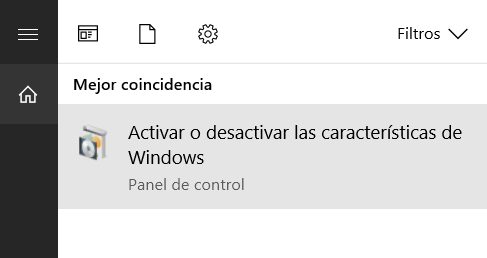
\includegraphics[width=8cm]{./Imagenes/1} 
\end{center}


\begin{itemize}
- Buscamos la opción llamada 'Hyper V', lo activamos la casilla y reiniciamos la pc.\\
\end{itemize}

\begin{center}
	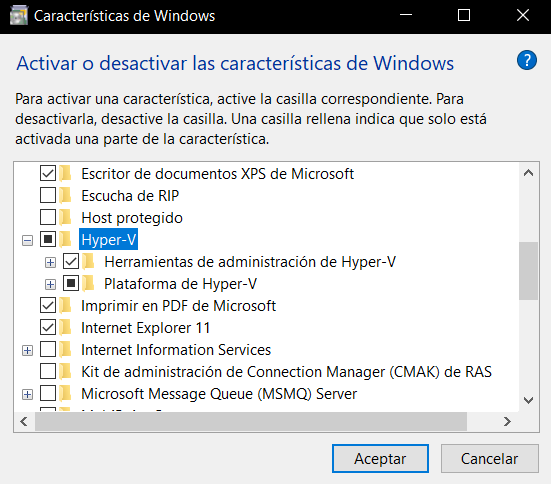
\includegraphics[width=8cm]{./Imagenes/2} 
\end{center}


\begin{itemize}
\subsection{Configuración del Hyper-V}\\
- Nos dirigimos a 'Administrador de conmutadores virtuales'. En la ventana que nos muestra
tenemos que elegir conmutador 'Interno', luego hacemos click en 'Crear conmutador virtual'.
\end{itemize}

\begin{center}
	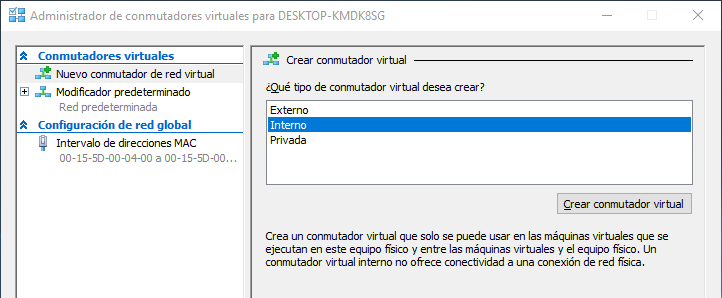
\includegraphics[width=10cm]{./Imagenes/3} 
\end{center}


\begin{itemize}
- Nos pedirá ingresar un nombre, ponemos el que deseamos. Verificamos si esta marcada la casilla
en 'Red interna' y damos click en 'Aceptar'.\\
\end{itemize}

\begin{center}
	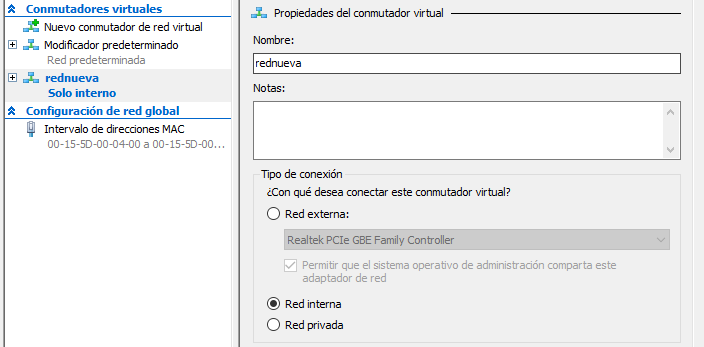
\includegraphics[width=10cm]{./Imagenes/4} 
\end{center}


\begin{itemize}

\subsection{Creación de la maquina virtual Ubuntu en Hyper-V}\\
- Hacemos click en 'Nuevo-Maquina virtual'. En la ventana que nos muestra ingresamos el nombre que deseemos poner a la maquina virtual, damos siguiente.
\end{itemize}

\begin{center}
	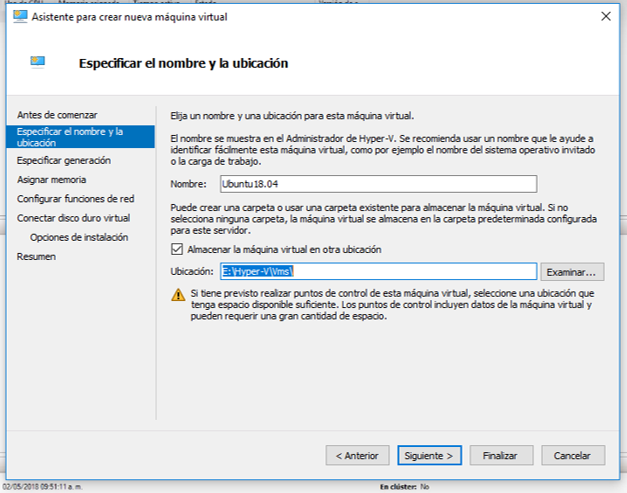
\includegraphics[width=10cm]{./Imagenes/7} 
\end{center}



\begin{itemize}
- Elegimos la generación 2\\
\end{itemize}

\begin{center}
	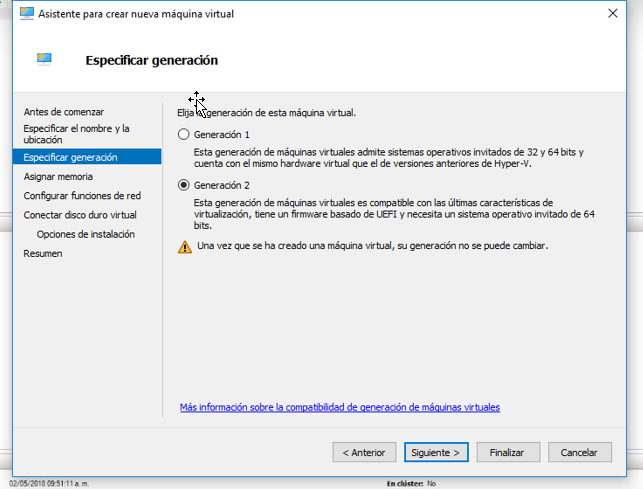
\includegraphics[width=12cm]{./Imagenes/8} 
\end{center}



\begin{itemize}
- Asignamos un total de 4096 MB de memoria RAM\\
\end{itemize}

\begin{center}
	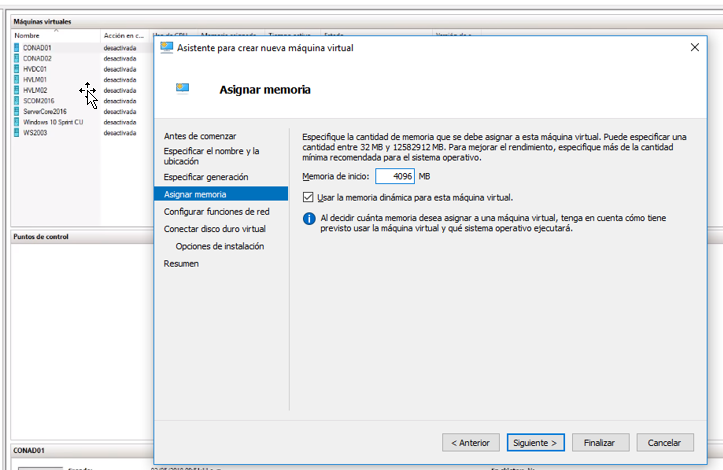
\includegraphics[width=12cm]{./Imagenes/9} 
\end{center}


\begin{itemize}
- En esta parte asignamos la red que hemos creado anteriormente, que en esta ocasión esta con el nombre de 'rednueva'\\
\end{itemize}

\begin{center}
	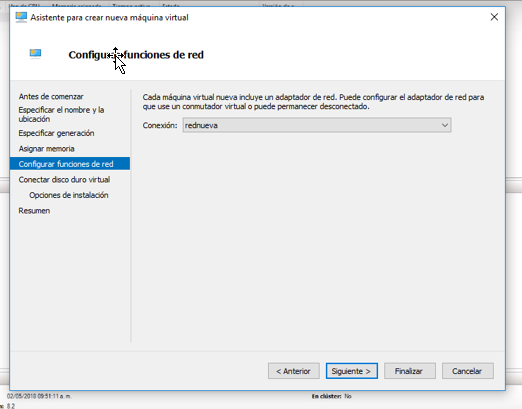
\includegraphics[width=12cm]{./Imagenes/10} 
\end{center}

\begin{itemize}
- En esta ventana escogemos la opción de 'Crear un disco duro virtual', en ubicación elegimos la carpeta donde querer guardar, damos click en siguiente.\\
\end{itemize}

\begin{center}
	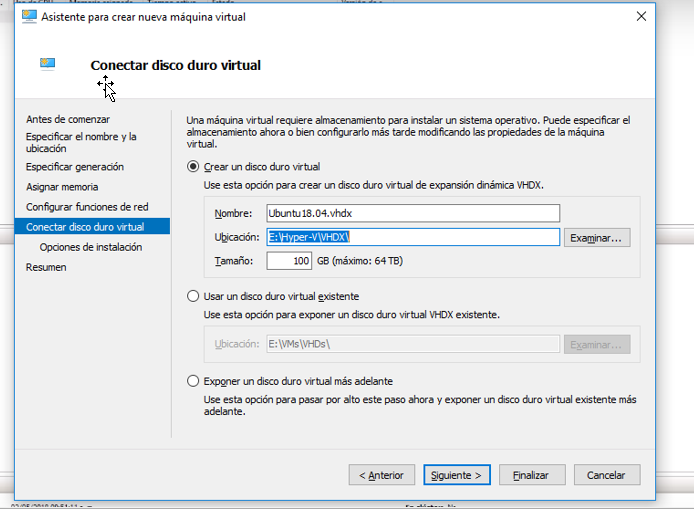
\includegraphics[width=12cm]{./Imagenes/11} 
\end{center}


\begin{itemize}
- En opciones de instalación seleccionamos la imagen .iso de Ubuntu\\
\end{itemize}

\begin{center}
	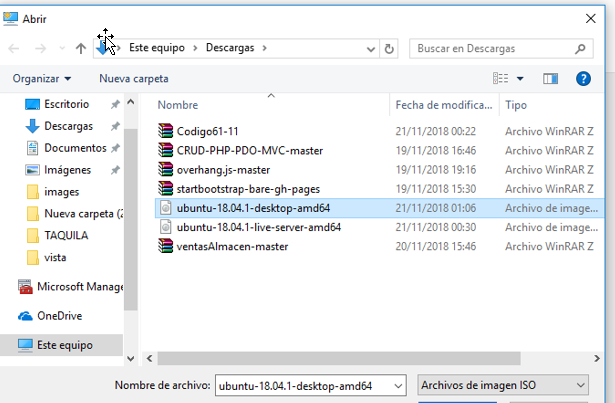
\includegraphics[width=12cm]{./Imagenes/12} 
\end{center}


\begin{itemize}
- Finalizamos la instalación de la maquina virtual\\
\end{itemize}

\begin{center}
	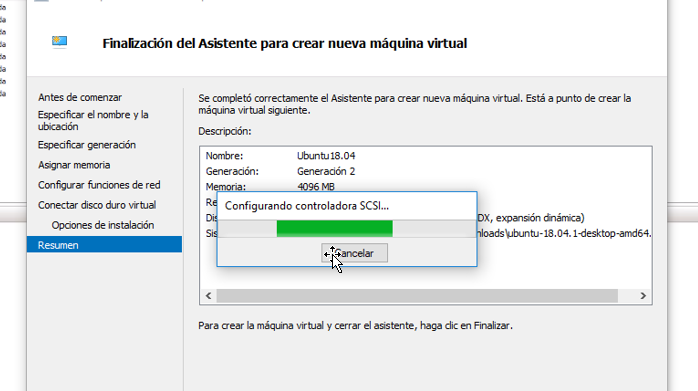
\includegraphics[width=12cm]{./Imagenes/13} 
	
\end{center}


\begin{itemize}
- Antes de iniciar la maquina virtual, vamos a la opcion de configuracion para desabilitar la siguiente opcion\\
\end{itemize}

\begin{center}
	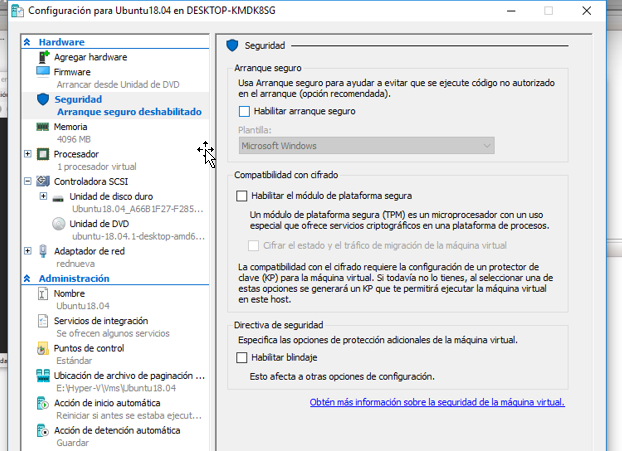
\includegraphics[width=12cm]{./Imagenes/14} 
\end{center}





\begin{itemize}
- Iniciamos la maquina virtual para poder terminar de instalar el sistema operativo Ubuntu, elegimos 'Install Ubuntu'\\
\end{itemize}

\begin{center}
	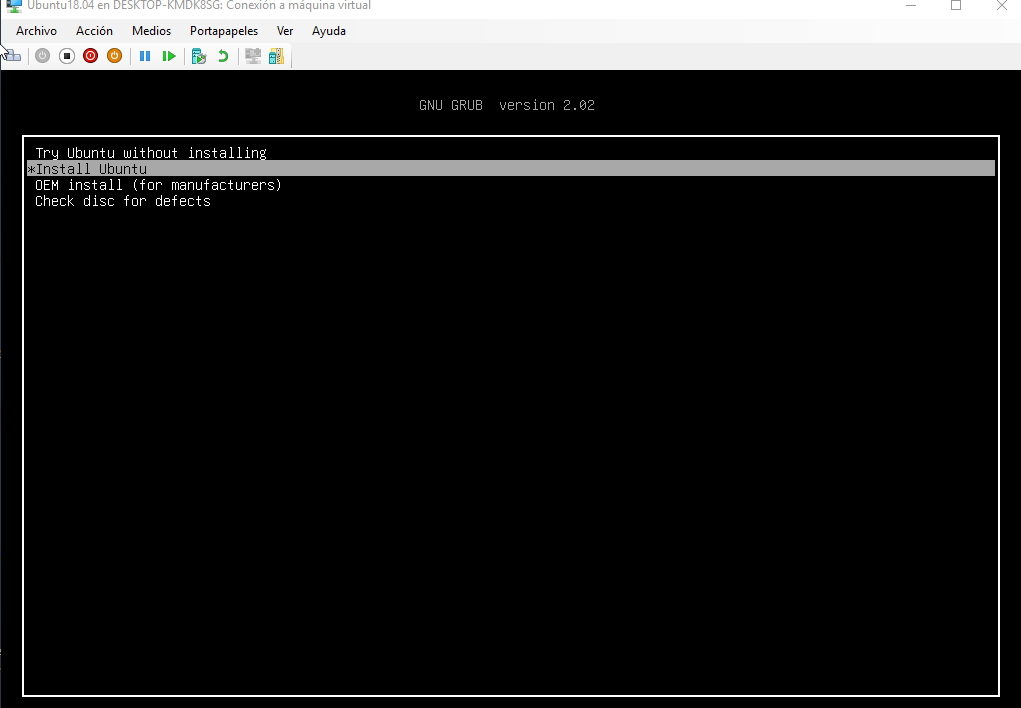
\includegraphics[width=12cm]{./Imagenes/15} 
\end{center}




\begin{itemize}
- Elegimos el idioma, damos continue\\
\end{itemize}

\begin{center}
	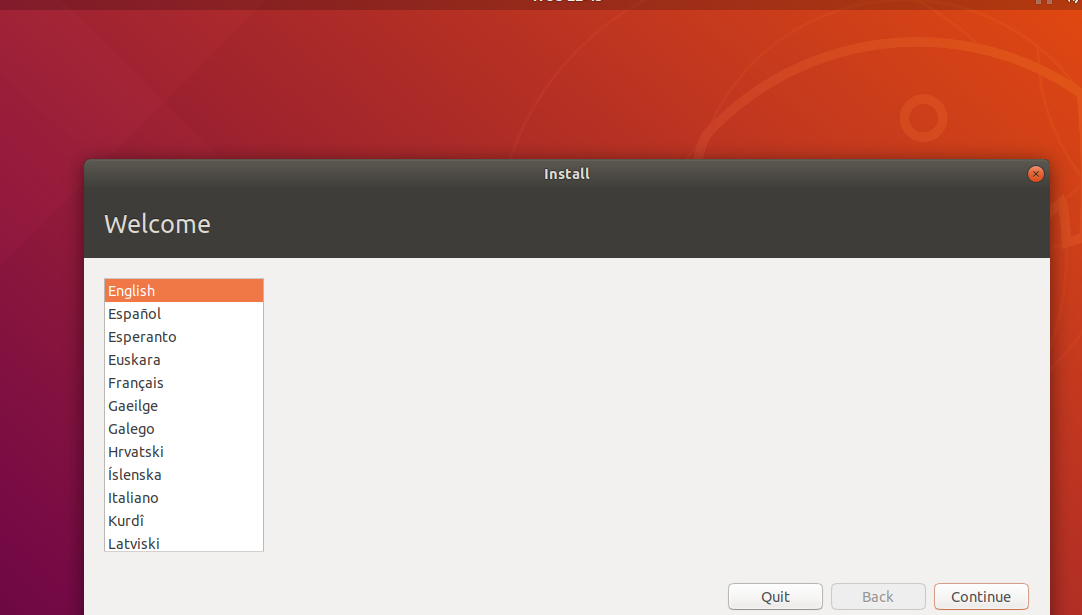
\includegraphics[width=12cm]{./Imagenes/16} 
\end{center}

\begin{itemize}
- Elegimos el idioma del teclado, damos click en continuar\\
\end{itemize}

\begin{center}
	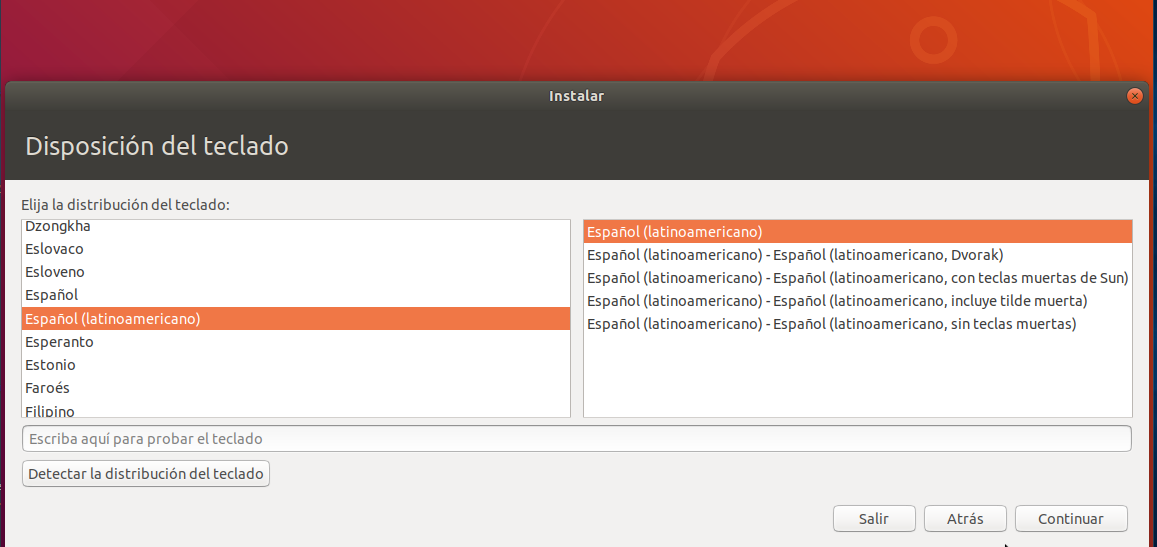
\includegraphics[width=12cm]{./Imagenes/17} 
\end{center}


\begin{itemize}
- En esta parte elegimos 'instalacion normal', damos click en continuar\\
\end{itemize}

\begin{center}
	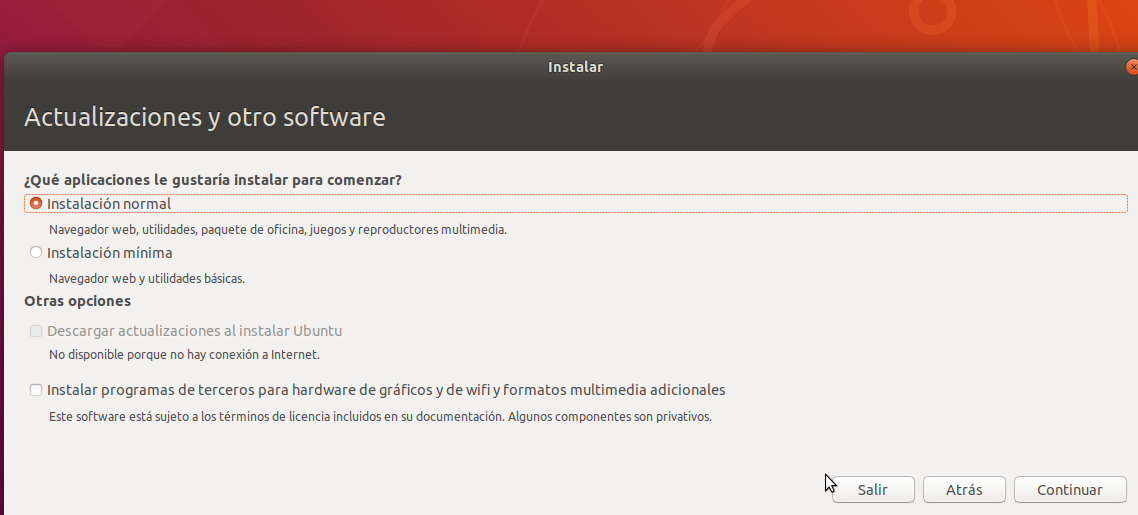
\includegraphics[width=12cm]{./Imagenes/18} 
\end{center}



\begin{itemize}
- Elegimos 'Borrar disco e instalar Ubuntu', y por ultimo damos click en instalar ahora\\
\end{itemize}

\begin{center}
	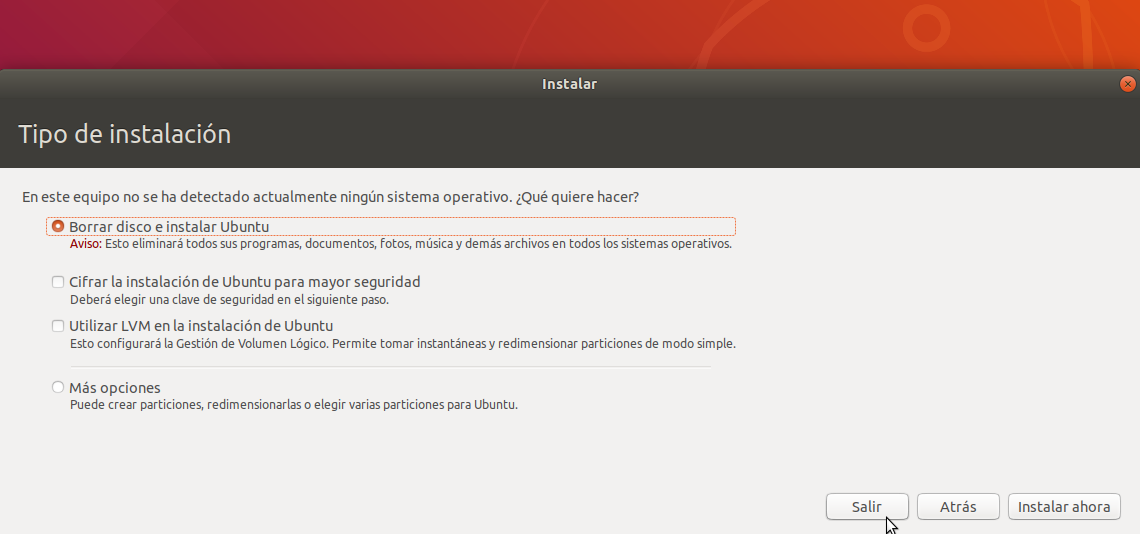
\includegraphics[width=12cm]{./Imagenes/19} 
\end{center}


\begin{itemize}
- Seleccionamos nuestra zona horaria, click en continuar\\
\end{itemize}

\begin{center}
	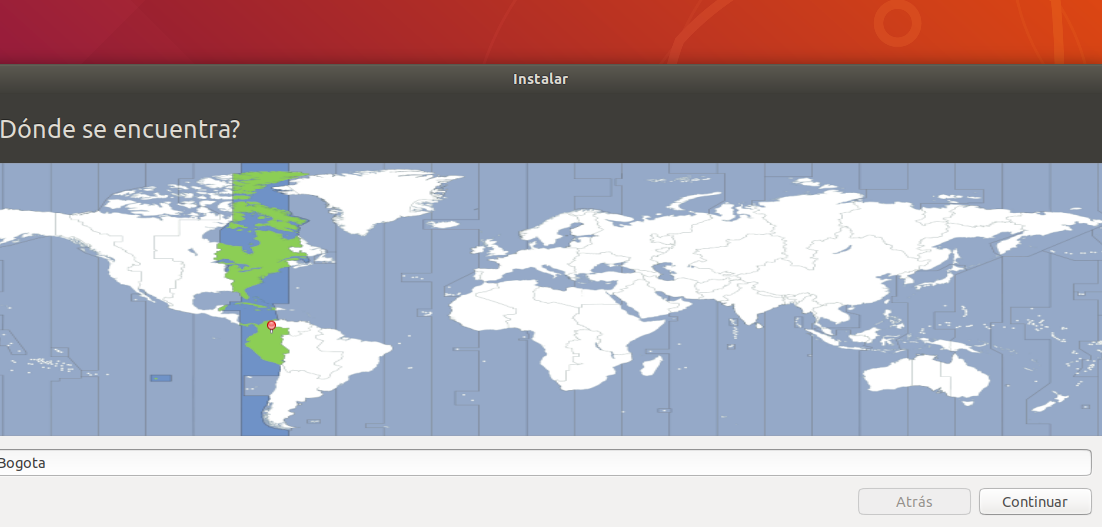
\includegraphics[width=12cm]{./Imagenes/20} 
\end{center}



\begin{itemize}
- Ponemos los datos necesarios que nos piden y esperamos q termine la instalacion\\
\end{itemize}

\begin{center}
	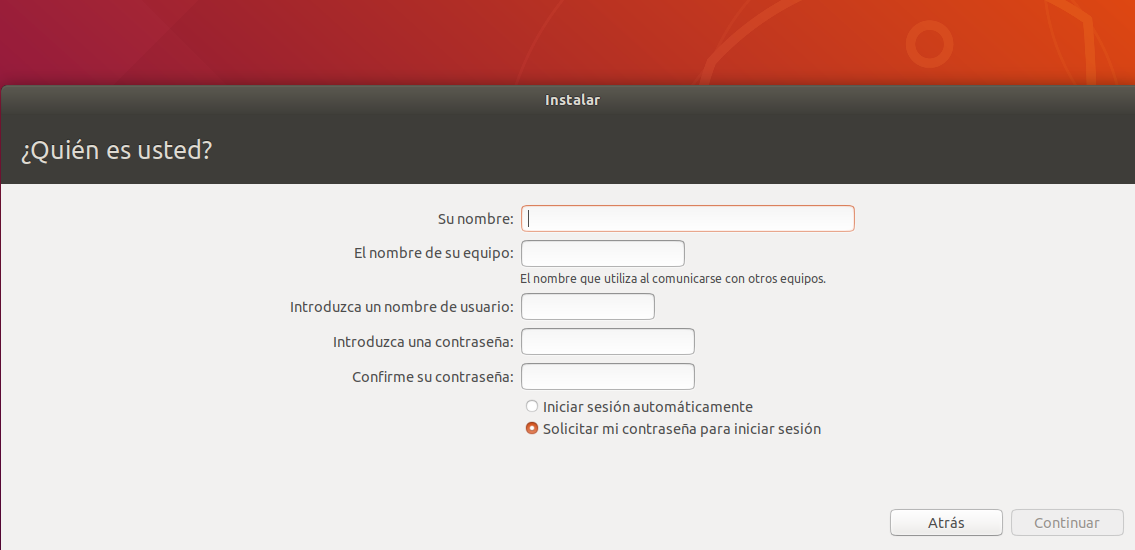
\includegraphics[width=12cm]{./Imagenes/21} 
\end{center}



\end{document}